\newpage
\null
\newpage
\section{Calculations for Graphene}
\label{sec:calculations}

The aim of this section is to model a three dimensional layer of graphene as depicted in figure \ref{fig:heeg-experiment} within the simulated data from section \ref{sec:simulation}. The geometry of this mesh is used to project the electric field $\mathbf{E}$ to the graphene layer and calculate the local and total enhancement of this layer.

The graphene layer is pulled into the cavity by about \SI{5}{nm} and spans over \SI{150}{nm} until reaching the substrate according to ref.~\cite{heeg}. To get a realistic estimation of the location of the graphene layer a 3D modelling software with cloth simulation will be used.

\subsection{Simulating the layer of graphene}

\begin{figure}[!h]
  \centering
  \begin{subfigure}{0.6\textwidth}
    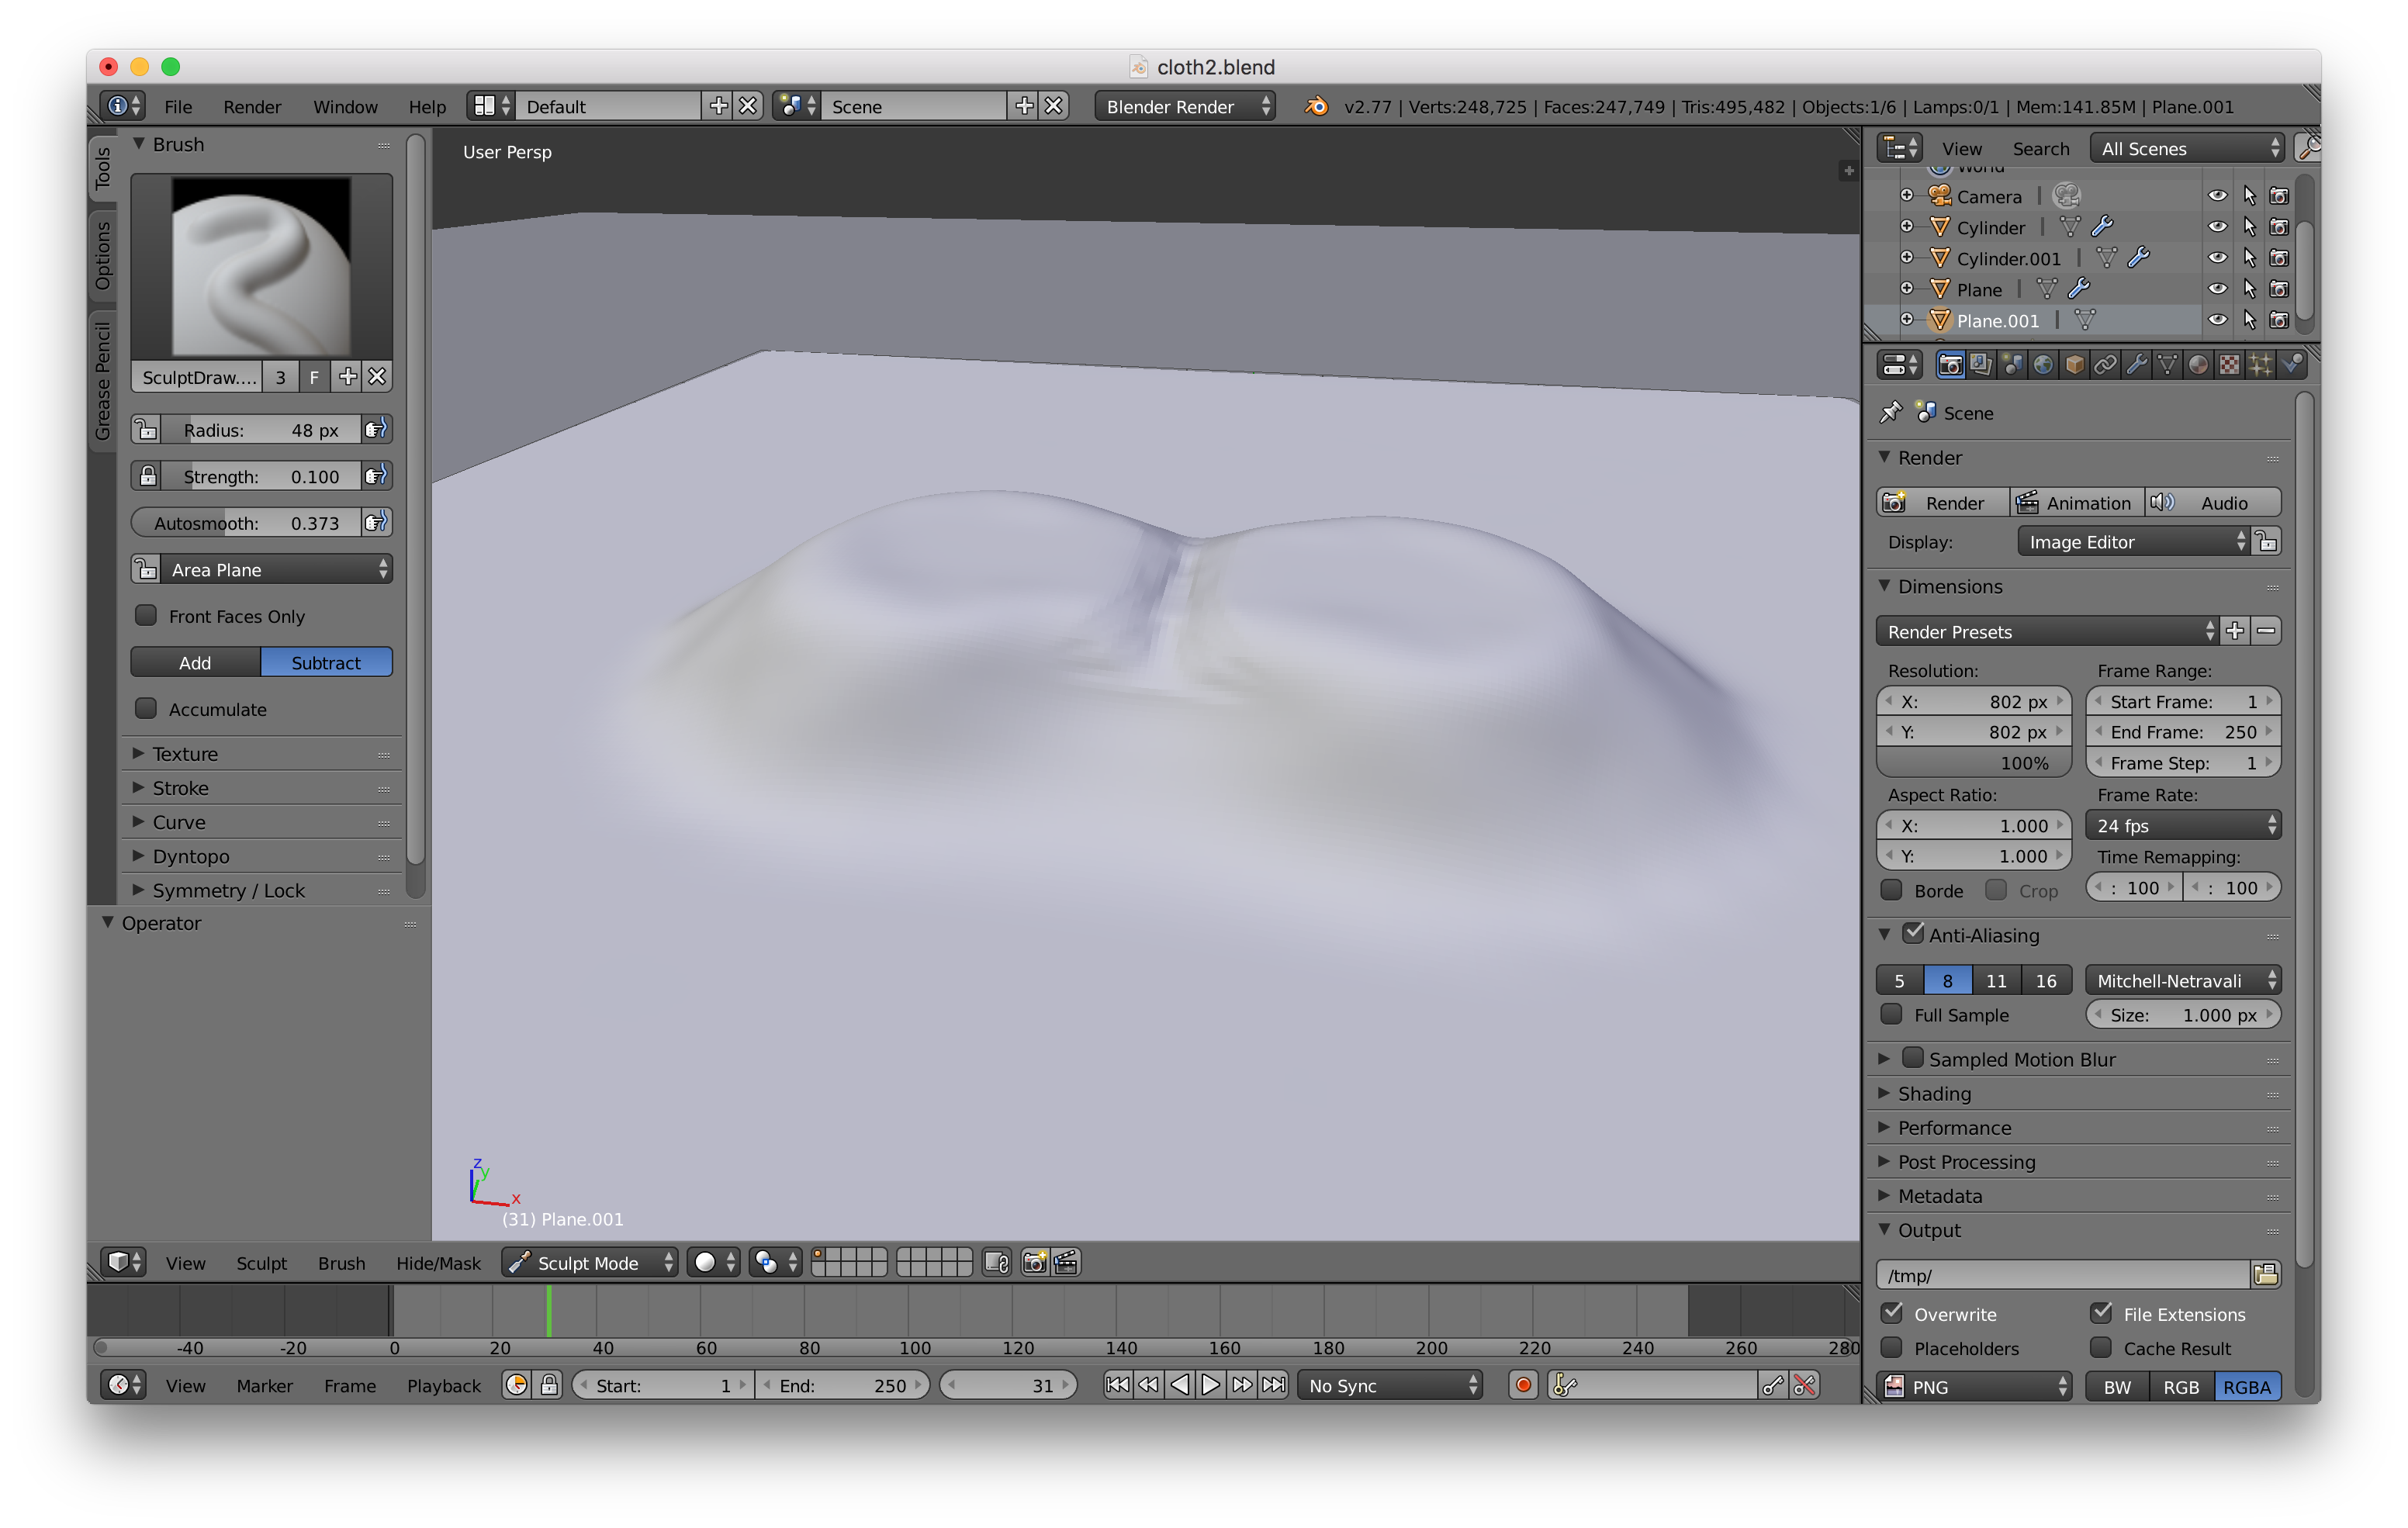
\includegraphics[width=\textwidth]{./images/blender.png}
  \end{subfigure}
  ~
  \begin{subfigure}{0.35\textwidth}
    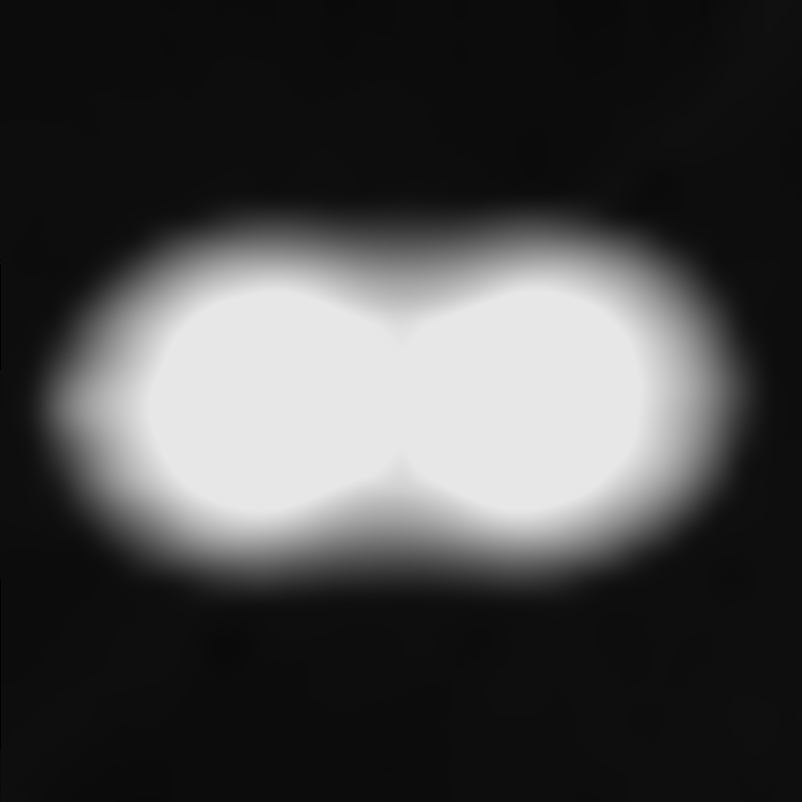
\includegraphics[width=\textwidth]{./images/map.png}
  \end{subfigure}
  \caption{\textbf{(a)} Cloth simulation in Blender 2.7. An elastic material is dropped on 2 cylinders with a radius of \SI{50}{nm}. \textbf{(b)} A generated heightmap after rendering. Black corresponds to 0, white to maximum height.}
  \label{fig:blender}
\end{figure}

Using the 3D modelling software Blender 2.7 a simulation of cloth falling on two cylinders was used to approximate the location of the graphene layer. As visible in figure \ref{fig:blender} two cylinders of \SI{45}{nm} height and \SI{50}{nm} radius (gold nanostructures plus chrome interlayer) were placed on an infinite plane. Next up a 1nm thick plane was placed on top and cloth simulation was enabled for this layer.

After the simulation finished with the cloth like material the results were compared to figure 1c of ref.~\cite{heeg}. This was repeated with tweeked properties of the material until the simulated 3D model matches the estimated position of the graphene layer. Because no material caused the layer to be pulled into the cavity the manual sculpturing tool was used to move the layer down into the cavity. The resulting 3D model is shown in figure \ref{fig:blender}.

To import the simulated structure into Matlab for further calculations an intermediate step is used. A camera is setup in the scene to point down at the structure with a special light source that illuminates the simulated layer according to it's $z$ value. The highest value is represented as white while black represents the base plane. All other values are projected linearly in the gray colorspace, effectively creating the heightmap shown in \ref{fig:blender}.

This heightmap can now be imported as a two dimensional matrix of height values:
\begin{minted}{matlab}
  classdef map
     properties
         values
     end
     methods
         function obj = map(name, scale)
            image = double(imread(name));
            if ndims(image) == 3
              image = 0.2989 * image(:,:,1) + 0.5870 * image(:,:,2) +
                0.1140 * image(:,:,3);
            end
            max_value = max(reshape(image, 1, []));
            obj.values = image ./ max_value .* scale;
         end

         function height = height(obj, x, y)
            height = obj.values(x, y);
         end
     end
  end
\end{minted}

This Matlab code imports an image, converts it to grayscale if needed, normalizes the values to be between 0 and 1 and then scales the heightmap with a factor. For a connection to the simulated near-field, the image has to have the same resolution as the simulation (401 datapoints in the $x$- and $y$ axis for this case). The normalization is needed to account for the height map conversion: Within the image data in the portable network graphics format, only values are saved as a range (white = 2, black = 0), therefore skewing the $z$ axis. The height scale factor within the import resolves this problem.

The calculation is using a scale factor of $47$ so that the graphene layer is hovering \SI{2}{nm} above the gold structure. This is done to mitigate the lightning effects at the discretised surface of the nanostructure.
